%-----------------------------------------------------------------------------
%
%               Template for sigplanconf LaTeX Class
%
% Name:         sigplanconf-template.tex
%
% Purpose:      A template for sigplanconf.cls, which is a LaTeX 2e class
%               file for SIGPLAN conference proceedings.
%
% Author:       Paul C. Anagnostopoulos
%               Windfall Software
%               978 371-2316
%               paul@windfall.com
%
% Created:      15 February 2005
%
%-----------------------------------------------------------------------------


\documentclass[10pt]{sigplanconf}

% The following \documentclass options may be useful:
%
% 10pt          To set in 10-point type instead of 9-point.
% 11pt          To set in 11-point type instead of 9-point.
% authoryear    To obtain author/year citation style instead of numeric.

\usepackage{amsmath}
\usepackage{graphicx}
\usepackage{graphics}
\usepackage{subfigure}
\usepackage{multirow}
\usepackage{rotating}
\usepackage{array}
%\usepackage{algorithmic}
%\usepackage{algorithm}
\usepackage{textcomp}
\usepackage{listings}
\usepackage{hyperref}
%\usepackage{url}
\begin{document}

%\conferenceinfo{SPLASH '11}{date, City.}
%\copyrightyear{2011}
%\copyrightdata{[to be supplied]}

\conferenceinfo{SPLASH'11 Companion,} {October 22--27, 2011, Portland, Oregon,
USA.}
\CopyrightYear{2011}
\copyrightdata{978-1-4503-0942-4/11/10}

\titlebanner{Crossfire Debugging Protocol}        % These are ignored unless
\preprintfooter{Crossfire - Multiprocess, Cross-Browser, Open-Web Debugging Protocol}   % 'preprint' option specified.

\title{Crossfire - Multiprocess, Cross-Browser, Open-Web Debugging Protocol}


\authorinfo{Michael G. Collins}
           {IBM Research - Almaden}
           {mcollins@collinsmichaelg.com}
\authorinfo{John J. Barton}
           {IBM Research - Almaden}
           {johnjbarton@johnjbarton.com}

\maketitle

%\begin{abstract}
This is an abstract.
\end{abstract}
\begin{abstract}
We present \textit{Crossfire}, a system and protocol designed to enable
debugging of Web pages in another process or machine. Issues specific to any one
Web browser are abstracted by the protocol and implementation,
allowing a new generation of Open Web development tools to be implemented. We discuss the major refactoring of Firebug, the open source Web debugging tool
to use \textit{Crossfire} and the interplay between goals and resources that such an effort requires.
In addition to the cross-browser focus of the protocol, we also discuss support for extensions which themselves will be
cross-browser and client-server.
\end{abstract}

\category{  D.2.5}{Software Engineering}{Testing and Debugging— debugging aids, distributed debugging}


\terms
Experimentation, Reliability

\keywords
Source-Level Debugging, Distributed Debugging, Open Source


\section{Introduction}
Web Applications continue to grow in size and complexity. Asynchronous background 
data download (AJAX) started the surge. 
This led to the 
emergence of common toolkits and libraries for Javascript which drove  performance
increases in Web Browsers fueling more growth in client-side Web application
development. These improvements, combined with new features available in Web browsers 
shifted investment from server- to client-side. Recent empirical analysis of representative
 major Web sites shows program sizes in the range of hundreds of kilobytes of
sophisticated code.\cite{VitekDynamicJS2010}

To develop and maintain these large applications, programmers and designers rely on 
numerous tools, most notably Web page debuggers. 
This paper describes a major re-architecting of the most widely used Web page debugger, 
Firebug, as a client/server system and in particular the 
\textit{Crossfire} protocol designed to support its client-server communications.  
Our description focuses on practical, state-of-the-art issues in an on-going and fast-moving project. 
Thus we cover details of protocol important for implementation and issues of 
matching resources to goals important for project management: we must deal with both 
extremes to succeed.

\section{Background}
To understand the importance and challenges of the \textit{Crossfire} work we start by introducing Firebug.
Released by Joe Hewitt in 2006, Firebug was the first integrated Web debugger. Firebug is a runtime 
debugger: it directly accesses, responds to, and operates on the running Web browser.  Rather than separate 
views of JavaScript, CSS, and HTML, Firebug integrated its views such that interaction with, 
for example, an HTML element would cause synchronized views of the CSS rules. Rather than static 
 views of browser state, Firebug included dynamics like network traffic analysis and console logging; rather 
than read-only views, Firebug allowed live edits where possible so developers could try out changes.
The resulting tool became very popular with developers and contributing significantly to the growth in Web applications.

The primary implementation of Firebug is a Firefox extensions, a supplemental software 
component that loads into the Firefox Web browser. A secondard implementation with fewer features and, 
in particular, limited support for JavaScript debugging, called Firebug Lite works in multiple browsers. 
The success of Firebug lead to implemenations of Web Page debuggers in other browsers, including 
DragonFly for Opera, Web Inspector for Google Chrome and Apple Safari, and the developer tool in 
Microsoft Internet Explorer. Since 2007 Firebug has been developed as an open source project, with 
seven major releases.

To give a flavor of the kinds of operations Firebug supports, we outline  an example more completely
described in Ref.\cite{jjb-www2010}. Suppose a developer wants to understand why a block of text 
in the Web page turned green while the page was loading. They might use the Firebug "inspect" feature, 
causing Firebug to display the HTML element under the mouse. They see that the element has a \textit{style}
attribute setting the color green. While hovering over the green block of text, 
the developer clicks down to lock
the user interface on the element, then moves to the HTML panel in Firebug and right clicks on the 
selected HTML element representation. A menu pops up allowing the developer to select "Break On Attribute Change". 
When the developer reloads the page, Firebug halts in the JavaScript code panel, on the line where 
the attribute is changed from red to green.

This example illustrates that we will need to synchronize mouse events on the Web page with the debugger UI,
identify HTML element representations rendered in the debugger UI with the elements in the Web page and synchronize
DOM mutation event handling wit JavaScript execution.


(Refactoring timeline)
=======
Web Applications continue to grow in size and complexity. The
emergence of common toolkits and libraries for Javascript along with performance
increases in Web Browsers fuels growth in client-side Web application
development. As more functionality shifts from server- to client-side, the size
of Javascript codebases naturally increases. Unfortunately for developers, the
tools to develop, manage, and debug larger codebases have not followed the
applications into the Web application development space.

Sophisticated development tools become crucial for understanding
and working with larger codebases. Compilers, debuggers, and other tools are
often combined to create an Integrated Development Environment (IDE) where
most, if not all, development tasks can be performed. Web development tools, on
the other hand, often reside in the Web Browser. In 2011, most Web
browsers ship with some kind of Web development tools included\cite{something},
and still more are available as plugins or add-ons. These tools operate
directly on the runtime Web application that is loaded into the browser, and do
not retain any knowledge of or connection to the original source code. Therefore
a developer must manually apply any changes made in one of these tools to his or
her source code.

This class of built-in Web development tools allow for a powerful set of
features.  However, several weaknesses.

Tools such as ``Inspectors'' and Firebug's HTML Breakpoints\cite{jjb-www2010}
enable developers to quickly locate the section of code they are interested in.

The rise of Mobile and Tablet computers which ship with fully functional Web
browsers means that Web application developers have additional form-factors to
consider.

Tools such as ``Inspectors'' and Firebug's HTML Breakpoints\cite{jjb-www2010}
enable developers to quickly locate the section of code they are interested in.

Crossfire is designed to support the features available in current built-in
development tools such as Firebug, while enabling the advantages of a remote
debug connection.



\section{Design Motivation}
\textit{Crossfire} has three main design goals: multiprocess support, remote and
mobile debug, and cross-browser debugging. These closely related goals arose out
of an interplay between user benefit and development costs. As an open source
project we must work with development resources motivated by goals: no matter
how much value Firebug users may receive from a goal, the selection must be
limited by the motivation of open source contributors.

Necessity motivated the first \textit{Crossfire} design goal, multiprocess
support. Soon after the Google Chrome browser was released, the Firefox team at
Mozilla began plans to convert Firefox to a multi-process design.  The Google
browser uses one controlling process for the application and one process for
each Web page.  This allows the browser to use the operating system isolation to
prevent problems on one page from bringing down the entire application and it
allows each page to use a different physical processor on modern multi-core
computers \cite{GoogleChrome}.  Depending upon the Firefox browser platform
changes, a shift to multiprocess could render a single-process Firebug debugger unusable.

 As a practical
matter we could not wait for the new platform to become available: with only
two full-time developers plus a number of dedicated but part-time contributors,
and a commitment to continuous compatibility with Firefox we had to begin work
immediately to ensure that our small resource could complete the transition in
time to remain a viable project.

Therefore we assumed that Firefox would eventually adopt
an architecture similar to Google Chrome: a client/server split debugger with a
back-end in one process and a front-end in another process.  We believe
that this assumption is planning for the worst case: converting Firebug to
client/server is a multi-person-year effort but likely to work with what
ever the Firefox team decides to do.

While necessity forced our action, opportunity followed. The client/server
choice, if successful, adds two new dimensions to Firebug for users: remote
debug and mobile device debug. We expect the value of these dimensions to grow
as more developers work in distributed teams and as mobile plays an increasingly
important role in Web application development.  In fact this value was
recognized by the DragonFly Web debugger for Opera\cite{opera-dragonfly} well before the Google
Chrome browser.\cite{WebInspector} The additional cost of designing for remote and mobile debug
on top of a client/server design -- primarily mechanisms for specifying the
connection addresses -- comes with potentially high benefits.  Moreover, the
benefits align with directions important to the project's primary open source
contributors (IBM and Mozilla).

The final goal of cross-browser debugging offers even more benefits to
Firebug users.  Web application developers by definition target all Web users,
but not all Web users are running identical Web platforms. Almost all
potential users of a Web site will be running one of few similar but slightly
different browsers. The commonality allows Web developers to do most of their
work on one browser, then test for differences on other browsers. Of course in
the latter case they need to debug the problem on a browser with unfamiliar debugging
tools. A common debugging tool across the major browsers would help with this
common and significant problem.

The benefit of cross-browser debugging comes at a high cost for the project.
Instead of one server and one client, we face at minimum one server for every
browser. And for each server we have to deal with both the slight differences in
browser implementation of standard Web APIs and potential large differences in
how debuggers can connect to the browser.


Unlike commercial or pure research projects, a community-driven open source
project like Firebug might balance the cost of implementing cross-browser debugging support by
attracting more contributors interested in this particular goal. That is, by
adding this costly goal we can attract new contributors, allowing us to create
more total value. In particular new contributors from the Orion
project\cite{orion}, joined to create a \textit{Crossfire} server for Microsoft
Internet Explorer and from the Eclipse project\cite{EclipseJSDT} to create a new
\textit{Crossfire} client in Java for connecting to Eclipse. Moreover, a
cross-browser client for Web debugging can be largely implemented with Firebug
Lite code, allowing our project to consolidate developer resources around fewer
lines of code to maintain.


Our three design goals created constraints for the \textit{Crossfire}
implementation. Above we outlined how the multiprocess support lead to a
client-server design choice. Support for remote and mobile debug forces
isolation of user interface to the client (excepting some small interface for
connection specification). The cross-browser goal creates constraints
indirectly: to minimize the extra cost of supporting multiple servers we chose
to adopt the Google Chrome communications channel (sockets) and wire protocol
format (JSON). Neither Firefox nor Internet Explorer had existing servers, so
they did not alter our choices. Opera had a server but no one on our open source
team planned to work with Opera and the server itself was not open source making
implementation more difficult.  Since Firebug is already written in JavaScript,
JSON format is especially easy to work with and has good performance\cite{json}.
 For the communications protocol, HTTP would be a better choice for the project:
the JavaScript support for HTTP is much better than sockets and HTTP works
better in practical remote scenarios through firewalls.  However we made the
judgment that better socket support was coming in the near
future\cite{websocketapi}, support was adequate now, and lowering cost on a
Google Chrome back-end was important.  In addition our goals imply that the
client and the communication protocol should be built from open Web standards to
maximize the reuse across target browsers.


\section{Evolution not Revolution}
In addition to motivating developers to contribute to \textit{Crossfire}, we
also need to motivate users to help us test and refine the system. As a
practical project supporting 3 million users, Firebug provides a large base of
experienced Web developers working with a broad spectrum of Web technologies. An
open source, working, state-of-the-art debugger motivates users to explain
problems, create test cases, provide documentation and to help other users with
problems that come up. To harness this
 unusual resource  for \textit{Crossfire} we need a plan for incremental
 refactoring of Firebug to be compatible
with \textit{Crossfire}.  The refactoring plan needs to provide waypoints for
the development and it needs to provide intermediate value to users and/or
contributors.


\subsection{Inter-application JavaScript Debugging}
The first intermediate state for \textit{Crossfire} is shown in Fig.\ref{fig:fireclipse}.
\begin{figure}[htp]
  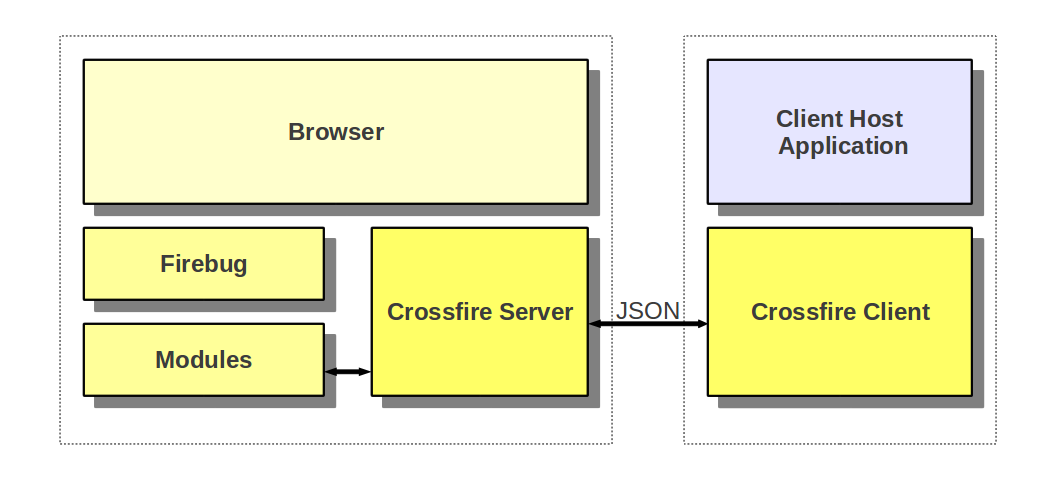
\includegraphics  [width = 86 mm] {figures/fireclipse.png}
  \caption{Inter-application JavaScript Debugging \textit{Crossfire} architecture.
\textit{Crossfire} versions 0.1 to 0.3 connected to an Eclipse plugin, supporting simple JavaScript debugging}
 \label{fig:fireclipse}
\end{figure}
In Firefox we implemented a \textit{Crossfire} server limited to support for JavaScript debugging.
In Eclipse we implemented a \textit{Crossfire} client. This allows the user interface in Eclipse to control
 and examine the JavaScript program running
in Firefox.  A proprietary version of the client shipped in IBM's Rational
Application Developer product for two years, then the open source Eclipse team created a new implementation as part of it's JavaScript Developer
Tools (JSDT) project\cite{EclipseJSDT}.  By working towards the Eclipse team's
goals of remote JavaScript debugging, this stage of the work provided valuable implementation
experience and engagement with the Eclipse team.
This work has been released to users but continues to be improved.

\subsection{Intra-browser JavaScript Debugging}
The second intermediate state implements the client side of the JavaScript part
of \textit{Crossfire} in a Web browser as sketched in Fig.~\ref{fig:fbugChrome}.
\begin{figure}[htp]
  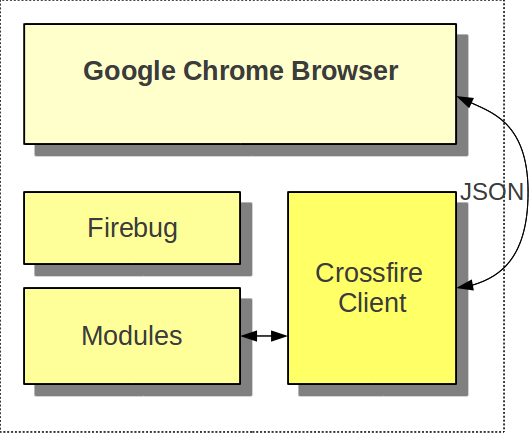
\includegraphics  [width = 86 mm] {figures/fbugChrome.png}
  \caption{Intra-browser JavaScript Debugging \textit{Crossfire} architecture.
\textit{Crossfire} versions 0.4 targets supporting simple JavaScript debugging with the client and server in the same application.}
 \label{fig:fbugChrome}
\end{figure}
While this diagram seems a bit bizarre, with the debugger running in and
connecting back into the the same browser, this step allows us to add JavaScript
debug support to the Firebug Lite implementation in the Google Chrome browser
while we simultaneously refactor the Firefox  \textit{Crossfire} server to
resemble the Google Chrome back end.


The key reason this architecture makes sense is that a large part of the
non-JavaScript parts of a Web page debugger uses standard Web APIs. That  means
that three different applications, Firebug Lite running as co-resident with a
Web page, Firebug Lite running as a Google Chrome extension,  and the
HTML/CSS/Console debug support code in Firebug for Firefox can use identical
code in different wrappers. By re-engineering our current somewhat divergent
code to group the identical parts we reduce maintainence. By adding
JavaScript debugging using the now platform-independent Firefox code to the
Firebug for Google Chrome code we add user value: the beginnings of cross
browser development. Both efforts contribute to our final goals.


Furthermore, the two JavaScript-only \textit{Crossfire} servers, one for Firefox
and one for Google Chrome, will be able to support alternative clients. In
particular, the Orion project, a Web based Web-development system, plans to
support JavaScript debugging over \textit{Crossfire} on their editor user
interface. In return that project is implementing a \textit{Crossfire} server
for Internet Explorer, allowing us to cover more than 75\% of the browser market
with \textit{Crossfire} supported tools. Versions with these features are scheduled
 to complete in
June, 2011.


\subsection{Cross-browser Debugging}
The final stage completes the transformation of an in-process single-browser Web
page debugger to a client-server cross-browser tool as shown in
Fig.~\ref{fig:crossbrowser}. \begin{figure}[htp]
  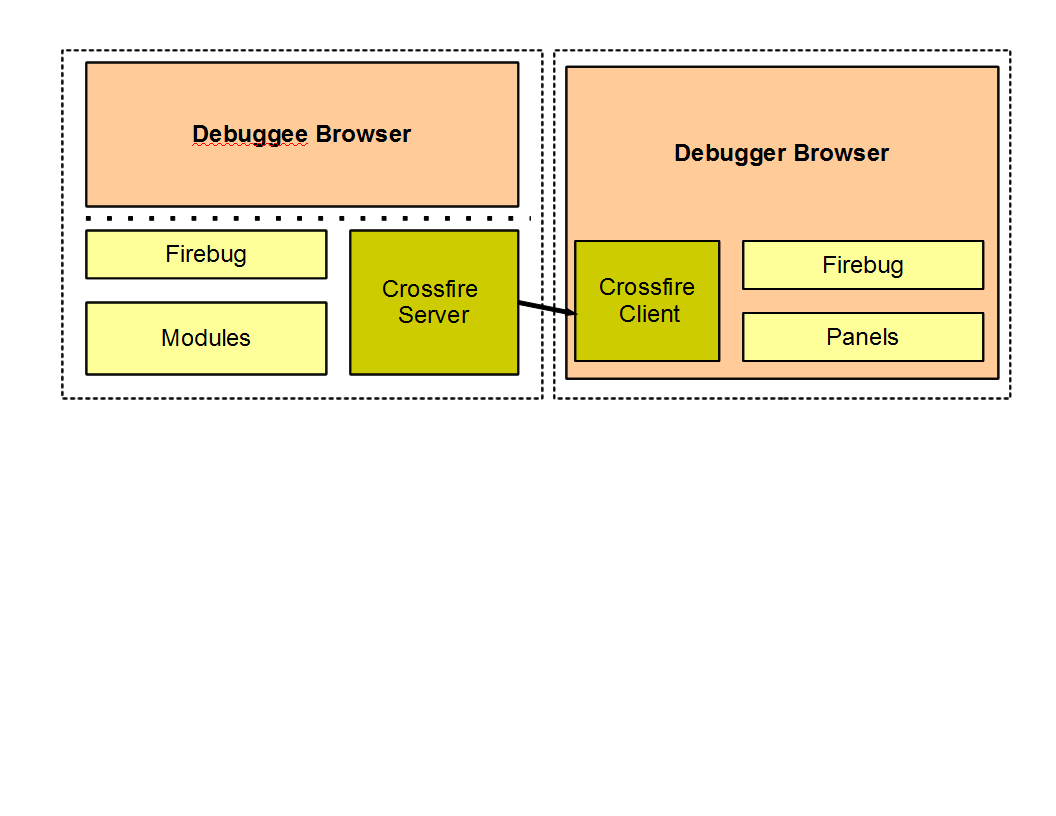
\includegraphics  [width = 86 mm] {figures/crossbrowser.png}
  \caption{Cross-browser Debugging architecture, proposed.}
 \label{fig:crossbrowser}
\end{figure}
Conceptually we simply re-apply the approach ironed out in the previous step to
the rest of the program and arrive at the complete value proposed at the outset.
In practice, the concept hides a lot of work. Many lines of code must be
carefully divide into two piles and the whole must be made to work again. This
work is scheduled to complete in Dec. 2011.

\subsection{Modules and Tools Interface}
In parallel with the architectural changes outlined above, we also need to make
important infrastructure improvements. Two such improvements are of particular
interest: conversion of the source code to 'modules' and introduction of a
cross-browser JavaScript tools application programming interface (API).


\paragraph{Modules} The original Firebug for Firefox and Firebug Lite code used
HTML \texttt{<script>} tags to load and compile the source. This approach has
two major drawbacks: 1) all of the top-level symbols in each file mix with the
top-level symbols of any other files loaded in the same scope and 2) the
load/compile steps are serialized. The first drawback never affected Firebug
code because all of the files encapsulated their symbols in function scope. But
the second one means that loading code always causes an upfront overhead to
starting the application.


A replacement for  \texttt{<script>} tag loading will need to support both
client and server sides of a refactored Firebug and it must allow us to debug
our own code.  As in other cases, we also want a solution that avoids additional
work by the development team. The solution we adopted was
\textit{RequireJS}\cite{requirejs}, a form of a module loader inspired by the
CommonJS\cite{commonjs} open standards effort.  For the client side or Firebug
Lite we can use this loader directly once we change our source to its format.
For the server side we needed to implement code to read source files within the Firefox
platform and to support debugging.


\paragraph{Tools Interface}
During the transformation from monolithic to client-server application, Firebug
needs to operate in both modes. The obvious way to deal with this is to
introduce a programming interface between the front and back ends. In Firebug
for Firefox, the interface functions call the back end directly; in the
intermediate and cross-browser version these functions
call the \textit{Crossfire} client API.  Similarly in the back end, the
multiprocess versions of the interface call the \textit{Crossfire} server.
Notice that this interface becomes a natural programming layer for interaction
between parts of the debugger. Since \textit{Crossfire} is designed to be
cross-browser, with some care in the design, the programming interface we create
becomes a general purpose Tools Interface for Open Web development.


The module and Tools Interface infrastructures complement one another. Each
logical chunk of the Tools Interface corresponds to the exported symbols from
one of the modules and the conditional assembly of the application from modules,
to become either in-process or client-server, works by using the module loader
to select the appropriate implementations of the interface.


\section {Protocol}
\subsection {Overview}
The Crossfire protocol is an asynchronous, bi-directional protocol designed to
enable the full functionality of the Firebug debugger in a multi-process or
remote scenario. Where it was possible, the design of the protocol took cues
from existing debug protocols such as DBGP\cite{dbgp}, Opera
Scope\cite{opera-scope}, Google's Chrome Dev Tools\cite{chrome-dev-tools} , as
well as common Web technologies (e.g. HTTP, JSON\cite{json}). Certain
features unique to Firebug and to debugging code running inside a Web Browser
had to be taqken into account in the design of the protocol.

Debugging the code that implements a Web page or Web application differs in some
significant ways from debugging applications developed for other systems.
HTML and CSS are used to declaratively specify the structure and style of the
user-interface, which is rendered by the Web browser. Developers cannot (easily)
debug the rendering code itself. Instead, built-in tools like Firebug allow the
developers to interact with the rendering engine by modifying the input and
observing the output in real time, via live CSS and DOM editing. JavaScript code
on the page can be stepped through when it is executing, however there is no
guarantee that any JavaScript code is necessarily running at any given moment.
JavaScript code on a Web page can be triggered by timers, user interactions or
network events. There is no outermost main or idle loop to return to; when a
section of JavaScript code is finished executing, control returns to the Web
browser. This confounds attempts at things such as a simple 'halt' command,
which is common among debuggers for other systems. The closest analog in Firebug
is the \textit{break-on-next} feature.

The Crossfire protocol is heavily event-driven, and requests made via Crossfire
are asynchronous. This differs from many other debug protocols which are often
synchronous or a combination of synchronous and asynchronous calls.  The reasons
for this decision stem from the nature of code running in a web page, and the
fact that in some scenarios, especially the intermediate scenarios we wished to
acheive, we would have a remote client connected to a server which also had a
co-resident debug UI (Firebug). In other words, a complete Firebug and Crossfire
server implementation would be running in a single Firefox process, and clients
could connect to the Crossfire server. The result of this scenario is that
clients cannot assume or rely on being the only agent acting on the runtime
engine. For instance, a Crossfire client cannot safely assume that the debugger
will remain suspended on a line of code until the client issues a request to
resume. It is also possible that this action was triggered by the user from
another client (in this case it is helpful to think of Firebug's in-process UI
as another client to the debugger). However any connected Crossfire client will
receive an event whenever the JavaScript debugger suspends or resumes, and
should react accordingly.

Implementations of the protocol differ based on whether the implementation is
intended to operate as a client or server. A Crossfire server resides in or is
connected to the process which is acting as the runtime platform for the Web
page, application, or other code which is to be debugged. This is typically a
Web Browser, although supporting other runtime environments is envisioned. A
Crossfire client connects to a server in order to receive events and issue
requests, typically in order to provide a user-interface
for debugging, (e.g. GUI or command-line debugger). It is not necessary for the
client and server to reside in the same process or even the same host machine.



%\begin{figure}[htp]
%  \includegraphics  [width = 86 mm] {figures/crossfire-example-packet.png}
%  \caption{An example of a Crossfire message packet.}
% \label{fig:crossfire-packet}
%\end{figure}
% \texttt{
% Content-Length:219
% \\r\\n\\r\\n
% {
%   "type":"request",
%   "command":"setbreakpoint",
%   "context_id":"http://localhost:8080/test.html",
%   "seq":21,
%   "arguments": {
%                  "position":0,
%                  "enabled":true,
%                  "target":"http://localhost:8080/test/some_javascript.js",
%                  "line":9,
%                  "ignoreCount":0,
%                  "type":"line"
%                }
% }
%\\r\\n
%}
\subsection {Client/Server Behavior}
Once a connection has been established and a successful handshake is completed,
the server may begin sending events to the connected client using the same TCP
connection used for the handshake. A client may also begin sending requests to
the server using the same connection. Clients should not expect the server to
respond synchronously to requests or in order. The most common example is a
Crossfire server sending one or more events to the client before responding to a
client's request, because the events occurred during the time the request was
being sent or processed.

\subsection {Extensibility}
One of the goals of Crossfire is to support remote and multi-process versions of
Firebug. One of Firebug's features is its ability to be extended, and there are
already many existing extensions. Therefore, we have developed what an API for
Crossfire, called the ``Crossfire Tools API''. The Tools API allows Firebug
extension developers a clean and consistent way to access the Crossfire client
and/or server connection.

On the server-side, the Tools API allows an extension to send custom events
and handle custom requests using Crossfire's connection and transport mechanism.
A client extension can listen for these events and respond to the requests.
Using this API, it will be possible for Firebug extensions to continue to adapt
to architectural changes in future versions of Firebug.

One consequence of this design choice is that the set of possible commands or
event names cannot be specified definitively by the protocol. A Crossfire
client or server must therefore be able to accept and respond to any well-formed
message packet, even if it may not know how to handle a particular command or
event type.

\subsection {Connection and Handshake}
Crossfire does not specify a standard or well-known port. Port agreement is left
up to the user, or the client software must start the server listening on
the same port it will attempt to connect to.

The Crossfire server listens for a TCP connection on the specified port
(greater than 1024).  A client wishing to connect sends the string
``CrossfireHandshake'' followed by a CRLF. The server replies with the same
string, at which point the connection is established and the client may begin
sending requests and receiving events from the server.

\subsection {Message Packets}
A well-formed Crossfire packet contains one or more headers consisting of the
header name, followed by a colon (``:``), the header value, and terminated by a
CRLF. A ``Content-Length'' header containing the number of characters in the
message body is required.

The message body is separated from the headers by a blank line
represented by a carriage-return character followed by a line-feed
character (CRLF).
The blank line should be followed by a well-formed JSON string, and terminated
by another CRLF. The message must contain a ``type'' field with the value one of
``request'', ``response'', or ``event'', and a ``seq'' field which contains the
sequence number of the packet. The sequence number of each message must always
be greater than that of the last message received.

\subsection {Contexts}
Firebug represents an instance of a Web page via an object called a
\textit{Context}. The context object allows Firebug's panels and modules to
share information about a web page that is being debugged, therefore it has a
central role in Firebug's architecture. The Crossfire protocol uses contexts for
most requests / events. Crossfire represents a context as a mapping of the
unique context ID and the URL of the page. This allows a connected Crossfire
client to distinguish between separate loads of the same URL, as is often the
case when a developer reloads a page several times in the course of developing
or debugging the page.
Firebug's TabWatcher component monitors loading and unloading of Firefox windows
and tabs.  The Crossfire server assigns a unique identifier to each
context, and passes this ID as part of most event and response packets.

\subsection {Context-specific events and requests}
Most of the events that occur in a Web browser that are of interest to a debug
UI are related to a single page. Examples of context-specific events include
loading (or reloading) of a page, loading and compiling a script, errors being
generated from an executing script, DOM elements being added or modified, a
breakpoint being added to a script, etc.

\subsection {Breakpoints}
Breakpoint debugging is a standard tool for debugging software at runtime in
many languages and environments. The Web Browser environment creates several
challenges for designing a remote protocol which supports breakpoint debugging.
Firebug also introduces several types of breakpoints which are not present in
other environments \cite{jjb-www2010}.

Even the simplest case, a JavaScript line breakpoint, has design implications
that must be considered. Typically, such a breakpoint is identified by a line
number and the URL of the script. However, existing JavaScript debugging APIs
such as Firefox's do not contain the concept of Firebug's contexts.  Therefore
if a user places a breakpoint on line 23 of a URL http://localhost/script.js,
then that breakpoint will exist for all occurrences of that URL. This may or may
not be what the user actually desires.  Considering the increasing use of
JavaScript libraries, it is entirely likely that a script from the same URL is
loaded into two completely unrelated pages. It is conceivable that a user would
wish to debug his or her code and the interaction with the library, without
affecting code running in another tab or window.

Crossfire's breakpoint protocol allows breakpoints to be set in one of two ways,
either with or without a context ID. If a Crossfire client specifies a context
ID along with a request to set a breakpoint, then that breakpoint should be
enabled only for that context, or a future context which is created with the
same URL in the same container (i.e. the page is reloaded).

If a client does not specify a context (by passing null as the value of the
context ID), then the behavior defaults to setting a breakpoint for the
specified location across all contexts, current and future.

More advanced breakpoints, such as the HTML element breakpoints, are supported
by specifying that the \textit{location} property of a breakpoint in Crossfire
is an arbitrary JSON object. A location object is defined depending on
the type of breakpoint.  A JavaScript line breakpoint has a location object
which consists of a target URL and line number. Firebug's HTML breakpoints have
a location object which consists of an XPath expression that identifies the
target element.  Eventually other location types may be added, e.g. to support
network-related breakpoints such as Firebug's \textit{BreakOnXHR} feature.

\section{Implementation}

\subsection{Crossfire Firefox Extension}
The first implementation of the Crossfire protocol is an extension implements
the protocol as an extension to Firefox and Firebug. The extension is
implemented entirely in JavaScript, using a modular design to allow us to share
code between client and server implementations, as well as cross-browser
implementations. This extension implements a flexible transport layer, allowing
the extension to operate as either a Crossfire client or server. This will also
enable both client and server to be implemented on top of other transport
layers, such as Web Sockets or HTTP.

The extension can be started in client or server mode either from the Firefox
user interface, or via command-line switches to Firefox. This latter mode of
operation allows external tools to launch Firefox and start the Crossfire server
listening on a known port so that the external tool may automatically connect
back to it. Figure \ref{fig:crossfire-arch}

\subsection{Crossfire Tools API}
The Crossfire extension also implements an API, called the ``Crossfire Tools API''
which enables extensibility of the Crossfire system and protocol. Firebug
features such as the Console, Inspector, and Net Panel, are implemented as tools
using the API, allowing them to be enabled/disabled independently.

\begin{figure}[htp]
  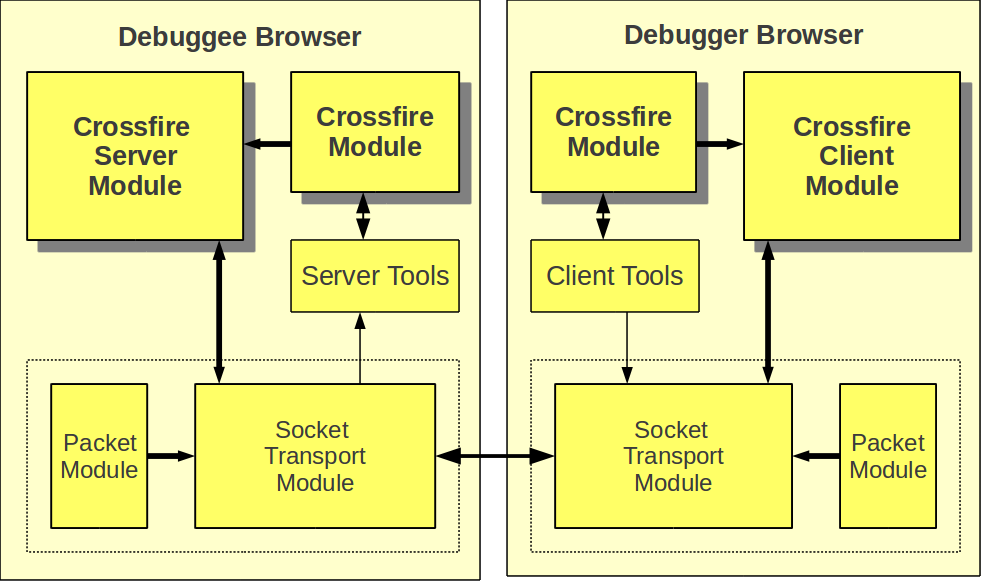
\includegraphics  [width = 86 mm] {figures/crossfire-arch4.png}
  \caption{Crossfire Firefox Extension Architecture}
 \label{fig:crossfire-arch}
\end{figure}

\subsection{Modules}

\subsection {Browser Tools Interface}

\section{Related Work}
\subsection{Multiprocess Web Debug Tools}
As we discussed above,
Opera's DragonFly\cite{opera-dragonfly} implements a complete remote debug
solution and Google Chrome's Web Inspector works across processes. These implementations are specific to their host browser.


\subsubsection{Weinre}
The Weinre (Web Inspector Remote)\cite{weinre} project implements a partial Web page debugger (no JavaScript debugging) by
adding JavaScript code to a Web page in a proxy server much like Firebug Lite. The
added code connects back to the proxy which then re-transmits to a third process running
the user interface code
from WebKit's Web Inspector. The main target for this work is mobile devices. If
a \textit{Crossfire} server were implemented in Weinre, the proxy could support connections to
 \textit{Crossfire} clients.

\subsubsection{Eclipse JSDT}
The Eclipse JavaScript Development Tools (JSDT) project\cite{EclipseJSDT}
includes a \textit{Crossfire} client implementation (currently in incubation).
 This code is written in Java and supports
connections to Firebug's server as well as an early implementation of \textit{Crossfire} in Internet Explorer.

\subsubsection{Orion}
The Orion project\cite{orion} aims to create Web development tooling based on
Web technologies, and plans to use Firebug and Crossfire as part of their
debugging support. Discussions with the Orion team helped inform the design of \textit{Crossfire}.

\subsubsection{Cloud 9 IDE}
The Cloud 9 IDE\cite{cloud9} supports remote JavaScript debugging (only) from a Web page to Google's V8
engine running in a \texttt{Node.js} server.

\subsection{Remote Protocols}
Many protocols have already been designed for the purposes of remotely debugging
an application running in another process, virtual machine, host, etc. The GNU
GDB debugger has an associated Remote Serial Protocol (RSP)\cite{gdb-rsp}. While
it is the only debugger we know of with its own song \cite{gdb-song}, it is
primarily designed for debugging native code, particularly on embedded
systems, and would not be well-suited for use with Firebug. The Java Debug Wire Protocol (JDWP)
\cite{jdwp} provides remote debugging of Java Virtual Machines. The protocol
supports command and response message pairs similar to Crossfire and other Web
debugging protocols. However the design of the protocol, particularly the
synchronous aspects, would not work well with Firebug's existing architecture.

\subsubsection{DBGp}
DBGp\cite{dbgp}, is an acronym for Debug Protocol, and was developed for version
2 of the XDebug debugger for the PHP language. Although it was designed not to
be language specific, many of the commands are intended to be synchronous, as
opposed to the asynchronous nature of Crossfire. DBGp also allows for the
debugger engine to send an event to a client via the 'notification' element,
with a custom body. However in order to support Firebug, we would need to define
the same events defined by Crossfire as DBGp notifications, essentially creating
another protocol within the protocol.

\subsubsection{Opera Scope Protocol}
The Opera browser has a built-in Web development tool called DragonFly, which
also supports the Scope remote debug protocol. The Scope
protocol\cite{opera-scope} supports XML and JSON formats, and features such as
JavaScript debugging and remote DOM inspection. It is used to allow the desktop
DragonFly client to connect to another Opera browser instance, including mobile
versions.

\subsubsection{V8 / Chrome Dev Tools Protocol}
The V8 protocol\cite{V8} is a JSON-based wire protocol for debugging JavaScript
programs running within the V8 engine. The Chrome Dev Tools
protocol\cite{chrome-dev-tools} wraps the V8 protocol to provide the additional
information needed to debug a Web page running within Google's Chrome browser.
The protocol implements JSON messages over TCP/IP sockets, and was the basis for
much of the initial work on the Crossfire protocol. However, over the course of
developing Crossfire and refactoring of Firebug, it was realized that Crossfire
would require more functionality than the Chrome protocols provided.



\section {Future Work}
\subsection {Web Sockets}
\subsection {Multi-user Debugging}
\section{Conclusion}
Our work thus far has demonstrated that it is possible to incrementally refactor
and rearchitect an existing codebase while maintaining the ability to support
Firebug's large user-base with releases which are compatible with new releases
of Firefox. In addition we have shown it is possible to implement a system for
remote debugging similar to existing solutions in other browsers, but using a
modular approach that is written purely in JavaScript. The project has been
successful in attracting new contributors and new opportunities for Firebug,
enabling the project to explore new directions. Continuing this work will
provide numerous benefits for Firebug users as well new features that are in
demand, while allowing Firebug to adapt to possible future changes in Firefox,
and increasing the features offered by Firebug/Firebug Lite in other Web
browsers.



\acks
As a multi-year open source effort, \textit{Crossfire} results from a broad collaboration and
contributions from many individuals. Simon Kaegi from the Orion team lead us towards collaboration with the Orion and Eclipse teams. Darin Wright wrote the initial implementation of the Tools Interface. Grant Gayed and Mike Rennie heavily influenced the \textit{Crossfire} protocol during their implementation of the IE server and Eclipse clients. Pedro Simonetti Garcia, Kevin Dangoor, and Atul Varma provided key insights to the module loading work. Jan 'Honza' Odvarko powers the Firebug project essential to our evolution strategy, especially implementing a test suite critical to maintaining the quality of the waypoint implementations. Steven Roussey helped with an early implementation and feedback on issues it raised.


% We recommend abbrvnat bibliography style.

\bibliographystyle{abbrvnat}

%\bibliography{bibliography}

% The bibliography should be embedded for final submission.

\begin{thebibliography}{27}
\providecommand{\natexlab}[1]{#1}
\providecommand{\url}[1]{\texttt{#1}}
\expandafter\ifx\csname urlstyle\endcsname\relax
  \providecommand{\doi}[1]{doi: #1}\else
  \providecommand{\doi}{doi: \begingroup \urlstyle{rm}\Url}\fi

\bibitem[web(2001)]{websocketapi}
Web{S}ocket {API} {S}pecification, 2001.
\newblock \url{http://dev.w3.org/html5/websockets/}.

\bibitem[jdw(2004)]{jdwp}
\emph{Java {P}latform {D}ebugger {A}rchitecture}, 2004.
\newblock \url{http://download.oracle.com/javase/1.5.0/docs/guide/jpda/}.

\bibitem[gdb(2007)]{gdb-song}
{GDB} {S}ong, 2007.
\newblock \url{http://www.gnu.org/music/gdb-song.html}.

\bibitem[chr(2009)]{chrome-dev-tools}
Google {C}hrome {D}ev {T}ools {P}rotocol, 2009.
\newblock
  \url{http://code.google.com/p/chromedevtools/wiki/ChromeDevToolsProtocol}.

\bibitem[Web(2010)]{WebInspector}
Web{K}it {W}eb {I}nspector, 2010.
\newblock \url{http://trac.webkit.org/wiki/WebInspector}.

\bibitem[clo(2010)]{cloud9}
Cloud 9, 2010.
\newblock \url{http://cloud9ide.com/}.

\bibitem[gdb(2010)]{gdb-rsp}
\emph{{GNU} {D}ebugger ({GDB}) {M}anual}, 2010.
\newblock \url{http://sourceware.org/gdb/current/onlinedocs/gdb/}.

\bibitem[ope(2010)]{opera-scope}
Opera {S}cope {P}rotocol, 2010.
\newblock \url{http://dragonfly.opera.com/app/scope-interface/}.

\bibitem[web(2010)]{websocketprotocol}
Web{S}ocket {P}rotocol, 2010.
\newblock \url{http://www.whatwg.org/specs/web-socket-protocol/}.

\bibitem[Ecl(2011)]{EclipseJSDT}
Eclipse {JSDT}, 2011.
\newblock \url{http://wiki.eclipse.org/JSDT/Debug}.

\bibitem[Goo(2011)]{GoogleChrome}
Google {C}hrome, 2011.
\newblock \url{http://www.google.com/chrome}.

\bibitem[IET(2011)]{IETools}
Microsoft {I}nternet {Explorer} {D}eveloper {T}ools, 2011.
\newblock \protect\url{http://msdn.microsoft.com/en-us/library/dd565628}.

\bibitem[V8(2011)]{V8}
V8 {D}ebug {P}rotocol, 2011.
\newblock \url{http://code.google.com/p/v8/wiki/DebuggerProtocol}.

\bibitem[com(2011)]{commonjs}
Common{JS}, 2011.
\newblock \url{http://www.commonjs.org/}.

\bibitem[cro(2011{\natexlab{a}})]{crossfire-doc}
Crossfire online documentation, 2011{\natexlab{a}}.
\newblock \url{http://getfirebug.com/wiki/index.php/Crossfire}.

\bibitem[cro(2011{\natexlab{b}})]{crossfire-src}
Crossfire source repository, 2011{\natexlab{b}}.
\newblock \url{http://fbug.googlecode.com/svn/extensions/crossfire/branches/}.

\bibitem[fir(2011{\natexlab{a}})]{firebug-doc}
Firebug developer api documentation, 2011{\natexlab{a}}.
\newblock \url{http://getfirebug.com/developer/api/firebug1.7/}.

\bibitem[fir(2011{\natexlab{b}})]{firebug-src}
Firebug source repository, 2011{\natexlab{b}}.
\newblock \url{http://fbug.googlecode.com/svn/branches/}.

\bibitem[get(2011)]{getfirebug}
Firebug website, 2011.
\newblock \url{http://getfirebug.com}.

\bibitem[ope(2011)]{opera-dragonfly}
Opera {D}ragon{F}ly, 2011.
\newblock \url{http://www.opera.com/dragonfly/}.

\bibitem[ori(2011)]{orion}
Orion, 2011.
\newblock \url{http://www.eclipse.org/orion/}.

\bibitem[Barton and Odvarko(2010)]{jjb-www2010}
J.~J. Barton and J.~Odvarko.
\newblock Dynamic and graphical web page breakpoints.
\newblock In \emph{Proceedings of the 19th international conference on World
  wide web}, WWW '10, pages 81--90, New York, NY, USA, 2010. ACM.
\newblock ISBN 978-1-60558-799-8.
\newblock \doi{http://doi.acm.org/10.1145/1772690.1772700}.
\newblock URL \url{http://doi.acm.org/10.1145/1772690.1772700}.

\bibitem[Burke(2011)]{requirejs}
J.~Burke.
\newblock Require{JS}, 2011.
\newblock \url{http://requirejs.org/}.

\bibitem[Caraveo and Rethans(2007)]{dbgp}
S.~Caraveo and D.~Rethans.
\newblock {DBGP, A common debugger protocol for languages and debugger UI
  communication, Draft 16}, 2007.
\newblock \url{http://www.xdebug.org/docs-dbgp.php}.

\bibitem[Crockford(2006)]{json}
D.~Crockford.
\newblock {JSON}, 2006.
\newblock \url{http://json.org}.

\bibitem[Mueller(2011)]{weinre}
P.~Mueller.
\newblock Weinre, 2011.
\newblock \url{http://pmuellr.github.com/weinre/ }.

\bibitem[Richards et~al.(2010)Richards, Lebresne, Burg, and
  Vitek]{VitekDynamicJS2010}
G.~Richards, S.~Lebresne, B.~Burg, and J.~Vitek.
\newblock An analysis of the dynamic behavior of javascript programs.
\newblock In \emph{Proceedings of the 2010 ACM SIGPLAN conference on
  Programming language design and implementation}, PLDI '10, pages 1--12, New
  York, NY, USA, 2010. ACM.
\newblock ISBN 978-1-4503-0019-3.
\newblock \doi{http://doi.acm.org/10.1145/1806596.1806598}.
\newblock URL \url{http://doi.acm.org/10.1145/1806596.1806598}.

\end{thebibliography}

\end{document}
